\documentclass{article}
  %----------------------------------------------------------------------------------------
%	Author:	WangYifu
%	Create Date:	2017-02-14
%	Last Modify:	2018-09-01
%----------------------------------------------------------------------------------------
\usepackage[T1]{fontenc}
\usepackage{fourier}
\usepackage[english]{babel}
\usepackage{amsmath,amsfonts,amsthm}
\usepackage{geometry}
\usepackage{fancyhdr}
\usepackage{listings}
\usepackage{color}
\usepackage[yyyymmdd]{datetime}
\usepackage{graphicx}
\usepackage{float}
\usepackage{titling}
\usepackage{titlesec}
%-------------------------------%
%          Page Style           %
%-------------------------------%
\pagestyle{fancyplain}
\fancyhead{}
\fancyfoot[L]{}
\fancyfoot[C]{}
\fancyfoot[R]{\thepage}
\renewcommand{\headrulewidth}{0pt}
\renewcommand{\footrulewidth}{0pt}
\setlength{\headheight}{13.6pt}
\textwidth=6.5in
\textheight=9.0in
\headsep = 0.1in
\renewcommand{\baselinestretch}{1.2}
\geometry{a4paper,left=2cm,right=2cm,top=2cm,bottom=2cm}

%-------------------------------%
%           Font Size           %
%-------------------------------%
\newcommand{\erhao}{\fontsize{22.1pt}{\baselineskip}\selectfont}
\newcommand{\sanhao}{\fontsize{16.1pt}{\baselineskip}\selectfont}
\newcommand{\sihao}{\fontsize{14.1pt}{\baselineskip}\selectfont}
\newcommand{\xiaosi}{\fontsize{12.1pt}{\baselineskip}\selectfont}
\newcommand{\wuhao}{\fontsize{10.5pt}{\baselineskip}\selectfont}
\newcommand{\setFontSize}[1]{\fontsize{#1}{\baselineskip}\selectfont}
\titleformat{\section}{\sanhao\bfseries}{$\bullet$}{5pt}{}

%-------------------------------%
%             Title             %
%-------------------------------%
\newcommand{\horrule}[1]{\rule{\linewidth}{#1}}
\renewcommand{\dateseparator}{ - }
\def\Assignment{Assignment Title}
\title{
\vspace{-2cm}
\normalfont \normalsize
\textsc{Washington University in St. Louis} \\ [0pt]
\horrule{1pt} \\[0.4cm]
\huge {\bf\Assignment}
}
\author{467261 - Yifu Wang}
\date{\normalsize\today\\\horrule{1pt} \\[0.5cm]}

%-------------------------------%
%           TableList           %
%-------------------------------%
\newcommand{\deflabel}[1]{#1\hfill}
\newenvironment{tlist}[1]{
	\begin{list}{}{
			\settowidth{\labelwidth}{\bf#1}
			\setlength{\leftmargin}{\labelwidth}
			\addtolength{\leftmargin}{\labelsep}
			\renewcommand{\makelabel}{\bf\deflabel}}}{
	\end{list}
}

%-------------------------------%
%             Code              %
%-------------------------------%
\definecolor{gray}{RGB}{191,191,191}
\definecolor{dkgreen}{RGB}{96,139,78}
\definecolor{mauve}{RGB}{206,145,120}

\lstset{ %
	language=C++,                % the language of the code
	% basicstyle=\textheight,           % the size of the fonts that are used for the code
	numbers=left,                   % where to put the line-numbers
	numberstyle=\color{black},  % the style that is used for the line-numbers
	stepnumber=0,                   % the step between two line-numbers. If it's 1, each line 
	% will be numbered
	numbersep=5pt,                  % how far the line-numbers are from the code
	backgroundcolor=\color{gray},      % choose the background color. You must add \usepackage{color}
	showspaces=false,               % show spaces adding particular underscores
	showstringspaces=false,         % underline spaces within strings
	showtabs=false,                 % show tabs within strings adding particular underscores
	frame=false,                   % adds a frame around the code
	rulecolor=\color{gray},        % if not set, the frame-color may be changed on line-breaks within not-black text (e.g. commens (green here))
	tabsize=2,                      % sets default tabsize to 2 spaces
	captionpos=b,                   % sets the caption-position to bottom
	breaklines=true,                % sets automatic line breaking
	breakatwhitespace=false,        % sets if automatic breaks should only happen at whitespace
	keywordstyle=\color{blue},          % keyword style
	commentstyle=\color{dkgreen},       % comment style
	stringstyle=\color{mauve},         % string literal style
}

  \def\Assignment{CES 417T - HW6}
  \usepackage[table,xcdraw]{xcolor}
\begin{document}
\maketitle
\begin{tlist}{3}
	\item[1.]
	Let denote C, S, T, P as Color, Stripes, Texture, Poisonous.
	\begin{tlist}{4}
		\item[(a)]
		$Entropy(P)=-\frac{3}{5}log_2\frac{3}{5}-\frac{2}{5}log_2\frac{2}{5}=0.673$\\
		$IG(C,P)=Entropy(P)-\frac{4}{5}(1)-\frac{1}{5}(0)=-0.127$\\
		$IG(S,P)=Entropy(P)-\frac{2}{5}(0)-\frac{3}{5}(-\frac{1}{3}log_2\frac{1}{3}-\frac{2}{3}log_2\frac{2}{3})=0.291103$\\
		$IG(T,P)=Entropy(P)-\frac{3}{5}(-\frac{1}{3}log_2\frac{1}{3}-\frac{2}{3}log_2\frac{2}{3})-\frac{2}{5}(1)=-0.109$\\
		So the root attribute of the tree will be Stripes.
		\item[(b)]
		Decision tree
		\begin{figure}[H]\centering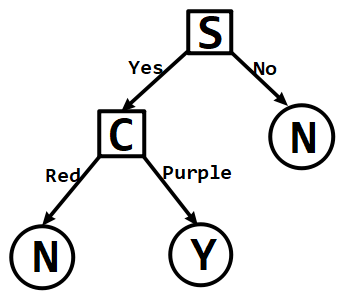
\includegraphics{1-b.png}\end{figure}
	\end{tlist}
	\item[2.]
	The 3-nearest neighbors are $(3,5);(3,8);(2,11)$, after regression we have $y=20-4.5x$, so $y$ will be $5.6$ when $x=3.2$.
	\item[3.]
	We have $$(+1,+1)\to(+1,+1):-1$$ $$(+1,-1)\to(+1,-1):+1$$ $$(-1,+1)\to(-1,-1):+1$$ $$(-1,-1)\to(-1,+1):-1$$
	That is
	\begin{figure}[H]\centering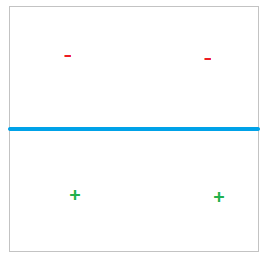
\includegraphics{3.png}\end{figure}
	The separator is $x_1x_2=0$, the margin is $1$. And drawing it back to original space. It will be the two axises.
	\begin{figure}[H]\centering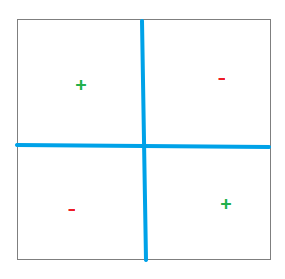
\includegraphics{3-2.png}\end{figure}
	\item[4.]
	\begin{align*}
		\|\Phi(x_i)-\Phi(x_j)\| & =\ \sqrt{\Sigma_{k=1}^D(x_{i,k}-x_{j,k})^2}                      \\
		                        & =\ \sqrt{\Sigma_{k=1}^D(x_{i,k}-x_{j,k})\times(x_{i,k}-x_{j,k})} \\
		                        & =\ \sqrt{K(x_i-x_j,x_i-x_j)}
	\end{align*}
	\item[5.]
	The true table will be
	\begin{center}
		\begin{tabular}{|c|c|c|c|}
			\hline
			\rowcolor[HTML]{C0C0C0}
			$x_1$ & $x_2$ & $x_3$ & $XOR(AND(x_1,x_2),x_3)$ \\ \hline
			+     & +     & +     & -                       \\ \hline
			+     & +     & -     & +                       \\ \hline
			+     & -     & +     & +                       \\ \hline
			+     & -     & -     & -                       \\ \hline
			-     & +     & +     & +                       \\ \hline
			-     & +     & -     & -                       \\ \hline
			-     & -     & +     & +                       \\ \hline
			-     & -     & -     & -                       \\ \hline
		\end{tabular}
	\end{center}
	That is $$g(\vec{x})=XOR(AND(x_1,x_2),x_3)=((\lnot x_1 \land x_3 )\lor(\lnot x_2 \land x_3)\lor(x_1 \land x_2 \land \lnot x_3))$$
	So the neural network will be($1$s are omitted)
	\begin{figure}[H]\centering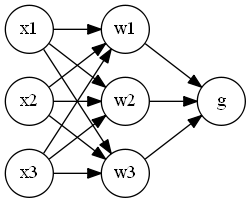
\includegraphics{5.png}\end{figure}
	Where
	\begin{align*}
		w_1 & =\ sign(-x_1+x_3-1.5)    \\
		w_2 & =\ sign(-x_2+x_3-1.5)    \\
		w_3 & =\ sign(x_1+x_2-x_3-2.5) \\
		g   & =\ sign(w_1+w_2+w_3+1.5) \\
	\end{align*}
\end{tlist}
\end{document}